\documentclass{article}

% Language setting
% Replace `english' with e.g. `spanish' to change the document language
\usepackage[english]{babel}

% Set page size and margins
% Replace `letterpaper' with `a4paper' for UK/EU standard size
\usepackage[letterpaper,top=2cm,bottom=2cm,left=3cm,right=3cm,marginparwidth=1.75cm]{geometry}

% Useful packages
\usepackage{amsmath}
\usepackage{graphicx}
\usepackage[colorlinks=true, allcolors=blue]{hyperref}

\title{TDT4171 — Artificial Intelligence Methods \\ Assignment 3 - Prob reasoning over time}
\author{Erik Storås Sommer - 535006}
\date{February 2023}

\begin{document}
\maketitle

\section*{Exercise 1}

\begin{itemize}
  \item The set of unobserved variables, denoted with \(X_t\), contains a single state variable \(Rain_t\) or \(R_t\) for short. It tells if it is raining or not.
  \item The set of observable variables, denoted with \(E_t\), contains a single evidence variable \(Umbrella_t\) or \(U_t\) for short. It tells weather someone has an umbrella or not. In the umbrella world, this is the director.
  \item Using the example from the book with the two states \(Rain=true\) and \(Rain=false\) we get the following dynamic model for \(P(X_t|X_{t-1})\):
  \[P(X_t|X_{t-1})= \begin{pmatrix} 0.7 & 0.3 \\ 0.3 & 0.7 \end{pmatrix}\]
  And observation model \(P(E_t|X_t)\):
  \[P(E_t|X_t)= \begin{pmatrix} 0.9 & 0.1 \\ 0.2 & 0.8 \end{pmatrix}\]
  where 0.9 is the probability of observing an umbrella when it is raining and 0.2 otherwise.
  \item The assumptions that are encoded in this model is that the current state of weather depends only on the previous state and not on any earlier states, where the states are days. This is therefor a first order Markov assumption. This assumption is reasonable since it does not take too many states into consideration. We have no information about where this is, and the location can have very large influence on the model and accuracy of the result.
\end{itemize}

\section*{Exercise 2}

The following figure shows the probability of rain at day 5 given the evidence of an umbrella at day 1, 2, 4 and 5. We also see that the desired probability of rain at day 2 is 0.883.

\begin{figure}[hbtp]
  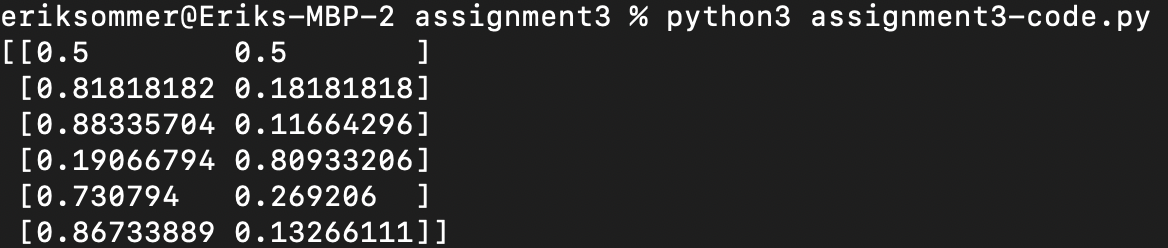
\includegraphics[width=\linewidth]{output.png}
  \caption{Output from running the attached python file}
  \label{fig:boat1}
\end{figure}

\end{document}